\documentclass[12pt]{exam}
%\documentclass[12pt]{article}
\usepackage[letterpaper, margin=0.75in]{geometry}
\usepackage{graphicx}
\usepackage{enumitem}
\usepackage{booktabs}
\usepackage{amsmath}
\usepackage{tabularx}
\usepackage{color}

\begin{document}
\footer{}{Page \thepage\ of \numpages}{}


\begin{center}

\includegraphics[width=10cm]{../images/logo.png}
\end{center}

\begin{center}
\noindent{\LARGE Conceptual Physics \\ Class 13 Questions \\ SOLUTIONS \\}
\end{center}
\vspace{0.5in}


\clearpage

\noindent\textbf{\Large Part 1: Probability}
\begin{questions}
	\question You have a jar with 73 red balls, and 27 blue balls. You randomly draw a ball from this jar. What is:
		\begin{parts}
			\part The percent chance that you will draw a red ball?
				\begin{TheSolution}
				There is a 73/(73+27) = 73/100 = 73\% change of drawing a red ball.
				\end{TheSolution}
			\part The percent chance that you will draw a blue ball?
				\begin{TheSolution}
				There is a 27/(73+27) = 27/100 = 27\% change of drawing a blue ball.
				\end{TheSolution}
			\part The probability that you will draw a red ball?
				\begin{TheSolution}
				P(red) = 0.73
				\end{TheSolution}
			\part The probability that you will draw a blue ball?
				\begin{TheSolution}
				P(blue) = 0.27
				\end{TheSolution}
			\part The probability of drawing a red or blue ball?	
				\begin{TheSolution}
				P(red or blue) = P(red) + P(blue) = 0.73 + 0.27 = 1
				\end{TheSolution}
		\end{parts}
		
	\question Give an example of 2 statistically \textit{independent} events.
		\begin{TheSolution}
			Rolling a die twice in a row. (Each roll is independent of the other)
		\end{TheSolution}
		
	\question Give an example of 2 statistically \textit{dependent} events.
		\begin{TheSolution}
		Drawing a card from the deck, and then drawing a second card from the (non-refilled) same deck.
		\end{TheSolution}
		
	\question You toss a coin in the air 3 times. What is the probability that:
		\begin{parts}
			\part It will land heads all 3 times?
				\begin{TheSolution}
				P(heads) $\times$ P(heads) $\times$ P(heads) = $1/2\times 1/2 \times 1/2$ = 1/8
				\end{TheSolution}
			\part It will land heads twice (and only twice)?
				\begin{TheSolution}
				The combinations that correspond to this are:
				HHT, HTH, THH which each have a probability of 1/8. The odds are therefore 1/8 + 1/8 + 1/8 = 3/8
				\end{TheSolution}
			\part It will land heads 2 or 3 times?
				\begin{TheSolution}
					The combinations associated with this are: HHH, HHT, HTH, THH each with probability 1/8. The sum is therefore 1/8+1/8+1/8+1/8=4/8=1/2 = 0.5
				\end{TheSolution}
			\part It will land tails 2 or 3 times?
				\begin{TheSolution}
					This is the same thing as asking head 2 or 3 times, since the coin is fair, therefore also 0.5
				\end{TheSolution}
		\end{parts}
		
\question You are tossing a fair coin, which has a 1/2 probability of landing heads and a 1/2 probability of landing tails. If you toss the coin in the air 300 times, how many times \textbf{on average} would you expect it to land:
	\begin{parts}
		\part Heads:
			\begin{TheSolution}
			You would expect half the time heads, and the other half the time tails: so on average 150 heads. This can also be done with the law of averages: $300\times 1/2 = 150$
			\end{TheSolution}
		\part Tails:
			\begin{TheSolution}
			This is the same as heads, since we are assuming a fair coin. 150
			\end{TheSolution}
	\end{parts}
\question You are tossing a trick coin, which has a 2/3 probability of landing heads, and a 1/3 probability of landing tails. If you toss the coin 300 times, hoe many times \textbf{on average}	 would you expect it to land:
	\begin{parts}
		\part Heads:
			\begin{TheSolution}
				\textbf{200} We expect it to, on average, be heads 2/3 of the time. 2/3 of 300 is 200.
			\end{TheSolution}
		\part Tails:
			\begin{TheSolution}
				\textbf{100} We expect it to, on average, be tails 1/3 of the time. 1/3 of 300 is 100.
			\end{TheSolution}
	\end{parts}
	
\question Based on your answers to the two previous questions, how could you tell if a coin was fair (without any special equipment or knowledge of how coins can be biased)?
	\begin{TheSolution}
		You could toss it 300 times. If it lands about heads 150 times, it is fair. If it lands about 200 times, then it is not fair. Note: The more times you toss it, the better statistics you get and the more certain you are of the answer.
	\end{TheSolution}
	
	\question There are 52 cards in a deck. You are dealt 2 cards (without refilling the deck). What is the probability that you will have both the ace of spades and the ace of diamonds?
		\begin{TheSolution}
There are two ways of looking at this. One is calculating the probability of drawing the ace of spades then ace of diamonds and the probability of drawing the ace of diamonds then ace of spades, and adding these probabilities since the two sequences of events are mutually exclusive. The other is to calculate the probability of drawing either the ace of spades or the ace of diamonds and then drawing whichever you didn't draw the first time.
\begin{eqnarray}
P(\text{ace of spades then ace of diamonds}) = \frac{1}{52}\cdot \frac{1}{51} = \frac{1}{2652} \nonumber \\
P(\text{ace of diamonds then ace of spades}) = \frac{1}{52}\cdot \frac{1}{51} = \frac{1}{2652} \nonumber \\
P((\text{spades then diamonds}) or (\text{diamonds then spades})) = \frac{1}{2652} + \frac{1}{2652} = \frac{1}{1326} \nonumber
\end{eqnarray}
For the second card, the probability goes up (the denominator goes down), because you are now drawing out of a deck of only 51 cards.

The other way of looking at it gives the same result:
\begin{eqnarray}
P(\text{ace of diamonds or spades then whichever card you didn't draw first}) = \frac{2}{52}\cdot\frac{1}{51} = \frac{1}{1326}\nonumber 
\end{eqnarray}

\end{TheSolution}
	
	\question Why isn't it valid to define randomness by saying that randomness is when all outcomes are equally likely?
		
	
	From \textit{Light and Matter}, Chapter 33 Discussion Question B
	\begin{TheSolution}
	Some events are more \textit{probable} than others. It is more probable to get heads when flipping an unfair coin than a fair one. These two situations are not the same, and this is reflected in the fact that different events occur with different likelihoods. This isn't to say the process isn't random, just that some events are more likely to happen than others.
	\end{TheSolution}
	
question Suppose you have two identical loaded four-sided dice, with $P(4) = 1/2$ and $P(1) = P(2) = P(3) = 1/6$.
		\begin{parts}
		\part If you rolled one die many times, what is the average value you would roll?
		\begin{TheSolution}
		The average value is the sum of each possible value times the probability of that value:
		\begin{eqnarray}
		1\cdot\frac{1}{6} + 2\cdot\frac{1}{6} + 3\cdot\frac{1}{6} + 4\cdot\frac{1}{2} = \frac{6}{6} + \frac{4}{2} = 3
		\end{eqnarray}
\end{TheSolution}
		\part If you rolled both dice, there are 16 possible rolls you could get. What is the probability of each?
		\begin{TheSolution}
		
		\begin{tabular}{l l l l}
		Roll & P(first roll) & P(second roll) & P(first and second roll) \\ \hline
		1, 1 & $\frac{1}{6}$ & $\frac{1}{6}$ & $\frac{1}{6}\cdot \frac{1}{6} = \frac{1}{36}$ \\
		1, 2 & $\frac{1}{6}$ & $\frac{1}{6}$ & $\frac{1}{6}\cdot \frac{1}{6} = \frac{1}{36}$ \\
		1, 3 & $\frac{1}{6}$ & $\frac{1}{6}$ & $\frac{1}{6}\cdot \frac{1}{6} = \frac{1}{36}$ \\
		1, 4 & $\frac{1}{6}$ & $\frac{1}{2}$ & $\frac{1}{6}\cdot \frac{1}{2} = \frac{1}{12}$ \\
		2, 1 & $\frac{1}{6}$ & $\frac{1}{6}$ & $\frac{1}{6}\cdot \frac{1}{6} = \frac{1}{36}$ \\
		2, 2 & $\frac{1}{6}$ & $\frac{1}{6}$ & $\frac{1}{6}\cdot \frac{1}{6} = \frac{1}{36}$ \\
		2, 3 & $\frac{1}{6}$ & $\frac{1}{6}$ & $\frac{1}{6}\cdot \frac{1}{6} = \frac{1}{36}$ \\
		2, 4 & $\frac{1}{6}$ & $\frac{1}{2}$ & $\frac{1}{6}\cdot \frac{1}{2} = \frac{1}{12}$ \\
		3, 1 & $\frac{1}{6}$ & $\frac{1}{6}$ & $\frac{1}{6}\cdot \frac{1}{6} = \frac{1}{36}$ \\
		3, 2 & $\frac{1}{6}$ & $\frac{1}{6}$ & $\frac{1}{6}\cdot \frac{1}{6} = \frac{1}{36}$ \\
		3, 3 & $\frac{1}{6}$ & $\frac{1}{6}$ & $\frac{1}{6}\cdot \frac{1}{6} = \frac{1}{36}$ \\
		3, 4 & $\frac{1}{6}$ & $\frac{1}{2}$ & $\frac{1}{6}\cdot \frac{1}{2} = \frac{1}{12}$ \\
		4, 1 & $\frac{1}{2}$ & $\frac{1}{6}$ & $\frac{1}{2}\cdot \frac{1}{6} = \frac{1}{12}$ \\
		4, 2 & $\frac{1}{2}$ & $\frac{1}{6}$ & $\frac{1}{2}\cdot \frac{1}{6} = \frac{1}{12}$ \\
		4, 3 & $\frac{1}{2}$ & $\frac{1}{6}$ & $\frac{1}{2}\cdot \frac{1}{6} = \frac{1}{12}$ \\
		4, 4 & $\frac{1}{2}$ & $\frac{1}{2}$ & $\frac{1}{2}\cdot \frac{1}{2} = \frac{1}{4}$
		\end{tabular}
\end{TheSolution}
		\part If you add up the values of your two rolls, you could get between 2 and 8. What is the probability of each possible sum?
		\begin{TheSolution}
		P(2) = P(1, 1) = 1/36
		
		P(3) = P((1, 2) or (2, 1)) = 1/36 + 1/36 = 2/36
		
		P(4) = P((1, 3) or (2, 2) or (3, 1)) = 1/36 + 1/36 + 1/36 = 3/36
		
		P(5) = P((1, 4) or (2, 3) or (3, 2) or (4, 1)) = 1/12 + 1/36 + 1/36 + 1/12 = 8/36
		
		P(6) = P((2, 4) or (3, 3) or (4, 2)) = 1/12 + 1/36 + 1/12 = 7/36
		
		P(7) = P((3, 4) or (4, 3)) = 1/12 + 1/12 = 1/6 = 6/36
		
		P(8) = P(4, 4) = 1/4 = 9/36

		The next part of the problem will be easier if we leave all the probabilities with the same denominator.
\end{TheSolution}
		\part What is the average sum you would get if you rolled both dice many times?
		\begin{TheSolution}
		\begin{eqnarray}
		2\cdot\frac{1}{36} + 3\cdot\frac{2}{36} + 4\cdot\frac{3}{36} + 5\cdot\frac{8}{36} + 6\cdot\frac{7}{36} + 7\cdot\frac{6}{36} + 8\cdot\frac{9}{36} = \nonumber \\
		 \frac{2+6+12+40+42+42+72}{36} = \frac{216}{36} = 6 \nonumber
		\end{eqnarray}
\end{TheSolution}
		
		\end{parts}

\question Does the number of radioactive nuclei in a sample decrease to exactly half its original value in one half-life? Explain in terms of the statistical nature of radioactive decay.
	\begin{TheSolution}
	No, one half-life is the time during which a radioactive nucleus will have a probability of 0.5 of decaying---on average, half the radioactive nuclei in a sample will decay during one half-life, but it is very unlikely that \textbf{exactly} one half the nuclei will decay. For example, a sample with one million radioactive atoms will decay to about 500,000 during one half-life, but the real number could be for example 500,012, or 499,987...it will probably not be precisely 500,000.
\end{TheSolution}
	
	\question Describe the following kinds of radioactive decay;
		\begin{parts}
			\part Alpha decay:
				\begin{TheSolution}
				A nucleus emits an alpha particle (helium-4 nucleus, which has 2 protons and 2 neutrons).
				\end{TheSolution}
				
			\part Beta decay:
				\begin{TheSolution}
				A neutron decays to form a proton, and in the process emits an electron (also called a beta particle)
				\end{TheSolution}
				
			\part Gamma decay:
				\begin{TheSolution}
					Highly energetic nuclei decay to less energetic states, and in the process emit a photon (gamma ray)
				\end{TheSolution}
		\end{parts}
		
	\question You have a block of radioactive material, and measure the number of initial decays to be 128 million. If it has a half-life of 4 hours, what do you expect its radioactivity level to be after:
		\begin{parts}
			\part 4 hours?
				\begin{TheSolution}
				\textbf{64.} This is 1 half-life, so you expect about 1/2 of the particles to remain: 128/2 = 64.
				\end{TheSolution}
			\part 8 hours?
				\begin{TheSolution}
					\textbf{16.} This is 2 half-lives, so you expect about $1/2\times 1/2 = 1/4$ of the particles to remain: 128/4 = 16.
				\end{TheSolution}
			\part 16 hours?
				\begin{TheSolution}
				\textbf{8.} This is 4 half lives, so you expect about $1/2\times 1/2\times 1/2\times 1/2=1/16$ of the particles to remain. 128/16 = 8
				\end{TheSolution}
		\end{parts}
		
	\question Does the number of radioactive nuclei in a sample decrease to exactly half its original value in one half-life? Explain in terms of the statistical
nature of radioactive decay.
	\begin{TheSolution}
	No, you expect about 1/2 to have decayed. This means if you have 100 identical samples, after 1 half life the average number of remaining particles will be 1/2 (but some samples may have slightly more, others may have slightly less).
	\end{TheSolution}
		
	\question What distinguishes between:
		\begin{parts}
			\item Different kinds of elements?
				\begin{TheSolution}
					Number of protons in the nucleus (different atomic numbers)
				\end{TheSolution}
			\item Different isotopes within an element?
				\begin{TheSolution}
					Number of neutrons in the nucleus (different atomic masses---the sum of protons and neutrons in the nucleus)
				\end{TheSolution}
		\end{parts}
		
	\question Physicists thought for a long time that bismuth-209 was the
heaviest stable isotope. (Very heavy elements decay by alpha emission because of the strong electrical repulsion of all their protons.)
However, a 2003 paper by Marcillac et al. describes an experiment
in which bismuth-209 lost its claim to fame — it actually undergoes
alpha decay with a half-life of $2\times 10^{19}$ years.
	\begin{parts}
		\part After the alpha particle is emitted (two protons and two neutrons), what is the isotope left over?
			\begin{TheSolution}
			An alpha particle is a helium-4 ion (two protons and two neutrons), so bismuth-209 decays to thallium-205.
\end{TheSolution}
		\part Compare the half-life to the age of the universe, which is about
14 billion years.
			\begin{TheSolution}
			14 billion years = $1.4\times 10^{10}$~years, so the half-life of bismuth-209 is about $10^9$ times longer than the age of the universe (about a billion times longer). Given this extremely long half life, it is not surprising that its decay was never observed before. According to the United States Geological Survey, the 2010 world mining output of bismuth was 8,900 metric tons, nearly all of which is bismuth-209. If the entire 2010 world output were stored for another 14 billion years, less than 4.5 grams of it would have decayed.
\end{TheSolution}
	\end{parts}
	
	\question What is the source of energy emitted in radioactive decay? (Hint: think about conservation laws from before)
	\begin{TheSolution}
		Nuclear potential energy.
	\end{TheSolution}
	
	\clearpage
	\noindent\textbf{\Large Part 2: Quantum Mechanics}
	
	\question What is the Heisenberg uncertainty principle?
		\begin{TheSolution}
			It is not possible, even in principle, to know the momentum and position simultaneously of a particle with perfect accuracy.
		\end{TheSolution}
	\question What is the concept of \textit{wave-particle duality}?
		\begin{TheSolution}
			Light an matter can exist both as waves and as particles.
		\end{TheSolution}
		
	\question How would the wavelength of an object change if:
		\begin{parts}
			\part Its mass increased?
				\begin{TheSolution}
				If the mass increased, the amount of energy that particle has would also increase. Therefore, the wavelength would decrease.
				\end{TheSolution}
			\part Its velocity decreased?
				\begin{TheSolution}
				If the velocity increased, the amount of energy that particle has would also decrease. Therefore, the wavelength would increase.
				\end{TheSolution}
		\end{parts}
		
	\question Three particles of equal mass are traveling in the same direction. The waves of
the three particles are as shown.
	\begin{center}
		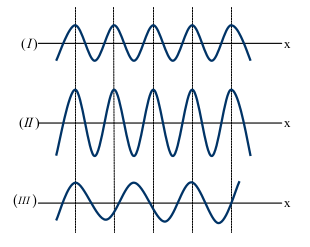
\includegraphics[width=3in]{../images/deBroglie.png}
	\end{center}
	Rank the speeds of the particles ( I ), ( II ) and ( III ) by circling one of these four possibilities.
\begin{choices}
	\choice $v_{II} > v_I > v_{III}$
	\choice $v_{II} > v_{III} > v_I$
	\choice $v_{I} = v_{II} > v_{III}$
	\choice $v_{II} > v_I = v_{III}$
\end{choices}
\begin{TheSolution}
\textbf{C.} Since they all have the same mass, we know that the larger velocity corresponds to larger energy. Energy is inversely proportional to the wavelength: the greater the energy, the smaller the wavelength. (I) and (II) have the same wavelength, and so must have the same velocity. (III) has a longer wavelength, and therefore less energy which means a longer wavelength.
\end{TheSolution}

	\question According to the uncertainty principle, the more we know about an electron's position,
the less we know about its
\begin{parts}
	\part speed.
	\part momentum.
	\part kinetic energy.
	\part all of these.
\end{parts}

	\question A metal surface is struck with light of wavelength 400nm, releasing a stream of electrons. If the 400nm light is replace by a 300nm light with the same number of photons incident on the metal per second, what will happen?
\begin{choices}
\choice More electrons are emitted in a given time interval
\choice Fewer electrons are emitted in a given time interval
\choice Emitted electrons are more energetic
\choice Emitted electrons are less energetic
\choice None of the above
\end{choices}
\begin{TheSolution}
\textbf{c}. Light of a shorter wavelength has a higher frequency and thus a higher energy.
\end{TheSolution}

\question A metal surface is struck with light of wavelength 400nm, releasing a stream of electrons. If the light intensity increases without changing the wavelength, what will happen?
\begin{choices}
\choice More electrons are emitted in a given time interval
\choice Fewer electrons are emitted in a given time interval
\choice Emitted electrons are more energetic
\choice Emitted electrons are less energetic
\choice None of the above
\end{choices}
\begin{TheSolution}
\textbf{a}. Increasing the intensity for a given wavelength means sending more photons; more electrons will be struck by photons and emitted from the surface.
\end{TheSolution}
	
	\question Why do we not notice quantum effects in our day-to-day lives?	
		\begin{TheSolution}
		Macroscopic objects consists of so many particles, and light beams of so many photons, that quantum effects average out to the classical limit.
		\end{TheSolution}
	
\end{questions}

\end{document}
